\section{Database}
Basis Data (database) adalah sebuah kumpulan data yang dapat disimpan secara terstruktur di dalam komputer untuk diolah atau di manupulasi menggunakan sebuah program aplikasi agar dapat menghasilkan informasi. Basis data ini merupakan bagian yang sangat penting dalam pembuatan sistem informasi karena berfungsi sebagai pusat penyimpanan data yang akan di organisasikan. Proses memasukan dan mengolah data dari media penyimpanan membutuhkan media perangkat lunak yang disebut DBMS (Database Management System). DBMS adalah sistem perangkat lunak yan dapat mengorganisasikan data secara praktis dan efisien.
\par
Beberapa perangkat lunak atau DBMS yang sering digunakan dalam pembuatan aplikasi antara lain:
\begin{enumerate}
\item MySQL - https://www.mysql.com/
\item Oracle - https://www.oracle.com/id/index.html
\item Microsoft SQL Server - https://www.microsoft.com/en-us/sql-server/sql-server-downloads
\item MariaDB - https://mariadb.org/
\end{enumerate}
Akan tetapi, dalam pembuatan aplikasi disini kita menggunakan MySQL.
\newline
MySQL adalah sistem manajemen basis data relasional open-source (RDBMS). Namanya adalah kombinasi dari "My", nama co-founder putri Michael Widenius, dan "SQL", singkatan dari Structured Query Language. MySQL adalah perangkat lunak bebas dan sumber terbuka di bawah ketentuan GNU General Public License, dan juga tersedia di bawah berbagai lisensi kepemilikan. MySQL dimiliki dan disponsori oleh perusahaan Swedia MySQL AB, yang dibeli oleh Sun Microsystems (sekarang Oracle Corporation). Pada 2010, ketika Oracle mengakuisisi Sun, Widenius melakukan forked pada proyek open-source MySQL untuk membuat MariaDB. MySQL adalah komponen dari tumpukan perangkat lunak aplikasi web LAMP (dan lainnya), yang merupakan akronim untuk Linux, Apache, MySQL, Perl / PHP / Python. MySQL digunakan oleh banyak aplikasi web berbasis database, termasuk Drupal, Joomla, phpBB, dan WordPress. MySQL juga digunakan oleh banyak situs web populer, termasuk Facebook, Twitter, Flickr, dan YouTube. 
\par
Untuk PHP kita menggunakan phpMyAdmin. phpMyAdmin adalah alat perangkat lunak gratis yang ditulis dalam PHP, dimaksudkan untuk menangani administrasi MySQL melalui Web. phpMyAdmin mendukung berbagai operasi di MySQL dan MariaDB. Operasi yang sering digunakan (mengelola basis data, tabel, kolom, hubungan, indeks, pengguna, izin, dll) dapat dilakukan melalui antarmuka pengguna, sementara Anda masih memiliki kemampuan untuk secara langsung menjalankan pernyataan SQL apa pun.
\subsection{SQL}
SQL (Structured Query Language) adalah bahasa standar untuk berkomunikasi dalam database. Menurut ANSI (American National Standards Institute) adalah bahasa standar yang digunakan untuk sistem manajemen basis data relasional. Pernyataan SQL ini dapat digunakan untuk melakukan perintah-perintah seperti memperbaharui dan mengambil data dari database. Beberapa sistem manajemen basis data relasional umum yang paling banyak digunakan adalah Oracle, Sybase, Microsoft SQL Server, Microsoft Access, dan masih banyak lagi.
\par
Terdapat 2 (dua) jenis perintah SQL, yaitu:
\begin{enumerate}
\item DDL (Data Definition Language), DDL adalah perintah SQL yang berhubungan dengan pendefinisian suatu struktur di dalam database. Perintah dasar yang termasuk DDL seperti:

\begin{itemize}
\item CREATE, Perintah yang digunakan untuk membuat database
\item ALTER, 
\item RENAME
\item DROP, 
\end{itemize}

\item DML (Data Manipulation Language), DML adalah perintah SQL yang digunakan untuk memanipulasi atau pengolahan data yang ada di dalam tabel. Perintah DML antara lain:

\begin{itemize}
\item SELECT
\item INSERT
\item UPDATE
\item DELETE
\end{itemize}
\end{enumerate}

\subsection{Membuat Database}
Untuk membuat database MySQL kita hanya menggunakan cmd atau command promt, yaitu:
\begin{itemize}
\item Disini kita dapat menekan tombol keyboard (windows + r) dan ketikan cmd dan muncul gambar

\begin{figure}[ht]
\centerline{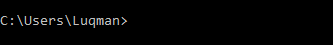
\includegraphics[width=1\textwidth]
{figures/cmd}}
\caption{}
\label{cmd}
\end{figure}

\item Jika sudah, selanjutnya kita ketikan perintah cd..

\begin{figure}[ht]
\centerline{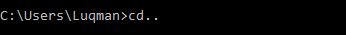
\includegraphics[width=1\textwidth]
{figures/cd1}}
\caption{}
\label{cd1}
\end{figure}

\item Tekan tombol enter, lalu ketikan perintah cd.. 

\begin{figure}[ht]
\centerline{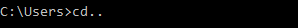
\includegraphics[width=1\textwidth]
{figures/cd2}}
\caption{}
\label{cd2}
\end{figure}

\item Setelah muncul, kita ketikan cd xampp/mysql/bin

\begin{figure}[ht]
\centerline{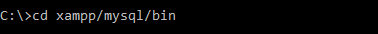
\includegraphics[width=1\textwidth]
{figures/cd3}}
\caption{}
\label{cd3}
\end{figure}

\item Setelah itu kita ketikan mysql -u root -p jika ada Enter Password enter saja karena secara default password kita kosong

\begin{figure}[ht]
\centerline{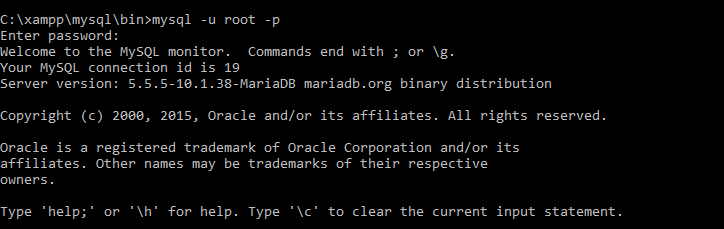
\includegraphics[width=1\textwidth]
{figures/cd5}}
\caption{}
\label{cd5}
\end{figure}

\item Jika sudah, kita dapat membuat database terlebih dahulu dengan mengetikan kode

\begin{lstlisting}
CREATE DATABASE php7;
\end{lstlisting}

\begin{figure}[ht]
\centerline{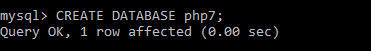
\includegraphics[width=1\textwidth]
{figures/cd6}}
\caption{}
\label{cd6}
\end{figure}

\end{itemize}

Bentuk perintah diatas digunakan untuk membuat sebuah database baru dengan nama php7. Aturan dalam penamaan pada umumnya database sama seperti aturan dengan penamaan sebuah variabel, kita bebas mengkombinasikan huruf, angka, dan underscore (\_). Akan tetapi, jika database yang akan kita buat sudah ada maka akan tampil pesan error.

\subsection{Menampilkan Database}
Untuk melihat apa saja database yang sudah kita buat dapat ketikan perintah sebagai berikut:
\begin{lstlisting}
SHOW DATABASES;
\end{lstlisting}

 \begin{figure}[ht]
\centerline{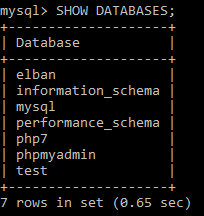
\includegraphics[width=1\textwidth]
{figures/show}}
\caption{}
\label{show}
  \end{figure}

\subsection{Membuka Database}
Kita harus membuka database MySQL yang ingin kita gunakan, atau mengaktifkanya dengan perintah USE. Silahkan ketik perintah sebagai berikut:
\begin{lstlisting}
USE php7;
\end{lstlisting}
Jika benar maka seharusnya tampil 'Database changed', artinya kita menggunakan database yang baru saja dibuat.
 \begin{figure}[ht]
\centerline{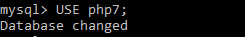
\includegraphics[width=1\textwidth]
{figures/use}}
\caption{}
\label{use}
  \end{figure}

\subsection{Menghapus Database}
Setelah perintah-perintah dasar mengenaii cara pembuatan database lalu bagaimana cara untuk menghapus database itu sendiri. Menghapus database menggunakan perintah DROP, perintah DROP digunakan untuk menghapus databse dan seluruh isi atau informasi yang ada di dalam database tersebut. Silahkan ketikan perintah sebagai berikut untuk menghapus database:
\begin{lstlisting}
DROP DATABASE php7;
\end{lstlisting}
Jika sudah benar, maka seharusnya akan tampil pesan sebagai berikut:
\begin{lstlisting}
Query OK, 0 rows affected (2.41 sec)
\end{lstlisting}
Jika memang sesuai maka itu artinya maka database kita sudah terhapus. Untuk lebih jelasnya silahkan lihat gambar berikut:
 \begin{figure}[ht]
\centerline{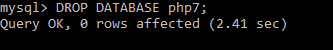
\includegraphics[width=1\textwidth]
{figures/drop}}
\caption{}
\label{drop}
  \end{figure}

\subsection{Membuat Tabel}
Untuk dapat membuat tabel kita harus pilih terlebih dahulu database mana yang akan kita gunakan. Contoh database yang akan kita gunakan adalah perusahan. Cara memilihnya kita gunakan perintah use.
\begin{lstlisting}
use nama_database
\end{lstlisting}
Karena kita akan menggunakan database perusahaan, maka kita mengetikan
\begin{lstlisting}
use perusahaan
\end{lstlisting}
Jika benar akan mucul tulisan database changed. setelah itu kita siap untuk membuat tabel. Struktur dalam pembuatan tabel sebagai berikut:
\begin{lstlisting}
Create table [nama tabel] (
nama field 1 type data,
nama field 2 type data,,
... nama field n);
\end{lstlisting}
Contoh apabila kita ingin membuat tabel dengan nama pegawai dengan 5 field sebagai berikut:
\begin{lstlisting}
CREATE TABLE pegawai(
id INT NOT NULL PRIMARY KEY,
nama_pegawai VARCHAR(30) NOT NULL,
jenis_kelamin VARCHAR(10) NOT NULL,
alamat VARCHAR(30) NOT NULL,
jabatan VARCHAR(20) NOT NULL
);
\end{lstlisting}
\begin{figure}[ht]
\centerline{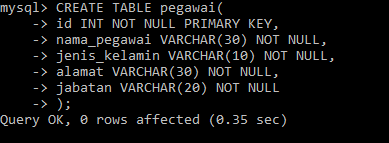
\includegraphics[width=1\textwidth]
{figures/create_table}}
\caption{}
\label{create}
\end{figure}
Untuk saran, penamaan tabel atau field jangan pakai spasi.

\subsection{Melihat Tabel}
Untuk melihat tabel kita dapat menggunakan perintah
\begin{lstlisting}
show tables;
\end{lstlisting}

Lalu untuk melihat isi dari tabel kita dapat meggunakan perintah
\begin{lstlisting}
desc [nama tabel];
\end{lstlisting}
Sebagai contoh kita menggunakan tabel pegawai maka perintahnya
\begin{lstlisting}
desc pegawai;
\end{lstlisting}

\begin{figure}[ht]
\centerline{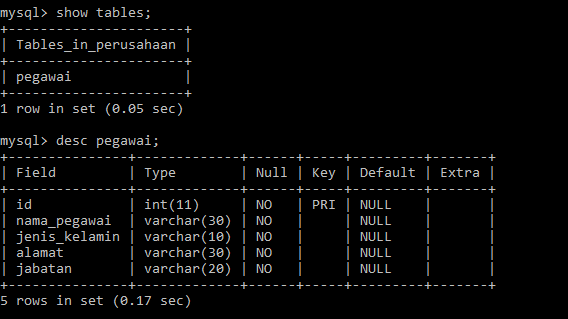
\includegraphics[width=1\textwidth]
{figures/lihat_tabel}}
\caption{}
\label{lihat}
\end{figure}






